The core idea of our this current section comes from following set of observations:
when working with \textit{PureCircuit}, one cannot fully work with binary logic, meaning
there is no trivial method for detecting $\bot$ values and removing them.
We therefore make use of topological problems with the idea that resolutions of our input
corresponds to some set nearby points in a space. If all points follows abide some property
then we can use that to detect solutions. We start with looking at the \textit{StrongSperner}
problem under the lens of \textit{Kleene logic}.
First we begin with the idea that solutions of \textit{StrongSperner} problems
revolve around the notion of panchromatic hypercubes. We can use the idea and make the following
definitions

\begin{definitionbox}{\textit{StrongSperner} anchor points}{ss-anchor}
    \label{def:ss-anchor}
    Given a hypercube $H \subset \mathbb{Z}^n$ of side lengths $1$, we denote
    the $\textbf{Anc}(H)$ as
    $$
        \textbf{Anc}(H) = \min_{p \in H} \|p\|_{1}
    $$
    Alternatively, we will refer to these hypercubes using the notation $\textbf{Cube}(\cdot)$ such that
    $$
        \textbf{Cube}(p) \triangleq \big\{(p + b) \mid b \in \{0,1\}^n \big\}
    $$
\end{definitionbox}

Ideally, we would like to express a cube as a coordinate of Kleene numbers, implying
the resolutions of the point will result in a hypercube, where each point is within
$\|\cdot\|_{\infty} \leq 1$ of each other.
An example of that can be seen in figure \ref{fig:chap-3:res-hyper}.
This leads to a natural interpretation of the \textit{StrongSperner} problem in \textit{Kleene logic}.
We will start with two definitions, one for \textit{nD-StrongSperner} and the other for
\textit{StrongSperner}. We remind that the main difference of the two problems is the former
has fixed dimensions $n$ of exponentially large cubes, whereas the other can have varying
dimensions of polynomially large widths.

\begin{figure}[h!]
    \centering
    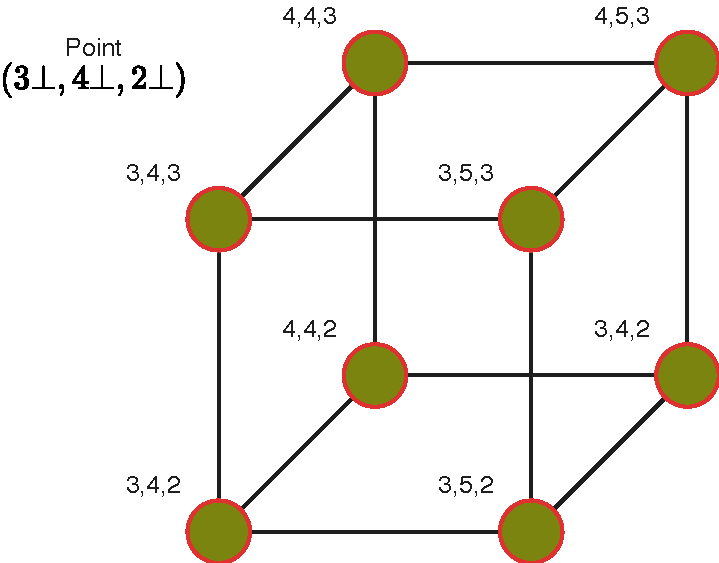
\includegraphics[width=0.3\textwidth]{Chapter3/1753903956-dissertation-drawing-assets.pdf}
    \caption{}
    \label{fig:chap-3:res-hyper}
\end{figure}


\begin{definitionbox}{\textit{HF-nD-StrongSperner} problem}{hf-nd-strong-sperner}
    \textbf{Input}: A circuit $\lambda: (\{0,1\}^k)^n \to \{-1, +1\}^n$, that describes a \textit{nD-StrongSperner} labelling,
    as explained in \ref{def:strong-sperner}, such that it is hazard free on inputs
    $(p_i\bot)_{i \in[n]}$ where $p_i \in \{0,1\}^{k-1 }$
    \textbf{Output}: A point $p \in \bigtimes_{i \in [n]} \left(\{0,1\}^{k-1} \times \{0,1 ,\bot\}\right)$ if and only if: $\lambda(p) =  \bot^n$.
\end{definitionbox}

We argue that the above problem is \textit{PPAD}-complete for all \textit{HF-nD-StrongSperner} problems. First we
can observe that all \textit{HF-nD-SS} are reducible to their \textit{nD-SS} counterparts since
hazard-free transformations have no effect on binary inputs and therefore our circuits acts like any other boolean circuit.
Chen et al. \cite{chen_SettlingComplexityComputing_2009} demonstated that for any $n \in \mathbb{N}$, \textit{nD-StrongSperner}
is \textbf{PPAD}-complete, and therefore \textit{HF-nD-StrongSperner} is in \textbf{PPAD}.
To show the hardness, we claim that
$$
    \textbf{PPAD}(\textit{nD-SS}) \subseteq \textbf{PPAD}(\textit{HF-nD-SS})
$$

\begin{proof}
    Given circuit $\lambda: (\{0,1\}^k)^n \to \{-1,+1\}^n$ from \textit{nD-SS},
    assume that $S$ is the set of anchors points of a panchromatic cube. We create
    $\Lambda: (\{0,1\}^{k+1})^n \to \{-1,+1\}^n$ such that:

    \begin{equation}
        \Lambda((x_{i})_{i \in [n]}) = \lambda\left( \left( { \left\lfloor \frac{x_{i}+1}{2}  \right\rfloor } \right)_{i \in [n]} \right) \label{eq:chap-3:trans-double}
    \end{equation}
    We prove the following claim

    \begin{claimbox}{Transformation claim}{trans-main}
        \label{clm:main-proof:trans-claim}
        Given $S_{\text{even}}$ the set of even solutions of the transformed space or more formally:
        $$
            S_{\text{even}} \triangleq
            \Big\{(p_i 0)_{i \in [n]}  \mid  p \in (\mathbb{B}^{(k)})^n:  (p_i 0)_{i \in [n]} \text{ is an anchor of a panchromatic cube} \Big\}
        $$
        We claim $|S| = |S_{\text{even}}|$
    \end{claimbox}

    \begin{proof}
        We argue that we can bijectively map between $S \leftrightarrow S_{\text{even}}$.
        To show the left to right direction, assume $p \in S$.
        Using figure \ref{fig:chap-3:dim-double} as reference, we can observe that each point becomes
        a $2^d$ hypercube. Essentially the hypercube that was anchored at $(p_1, ..., p_n)$ is mapped to
        the hypercube anchored at $(2p_1, ..., 2p_n)$.

        \begin{figure}[h!]
            \centering
            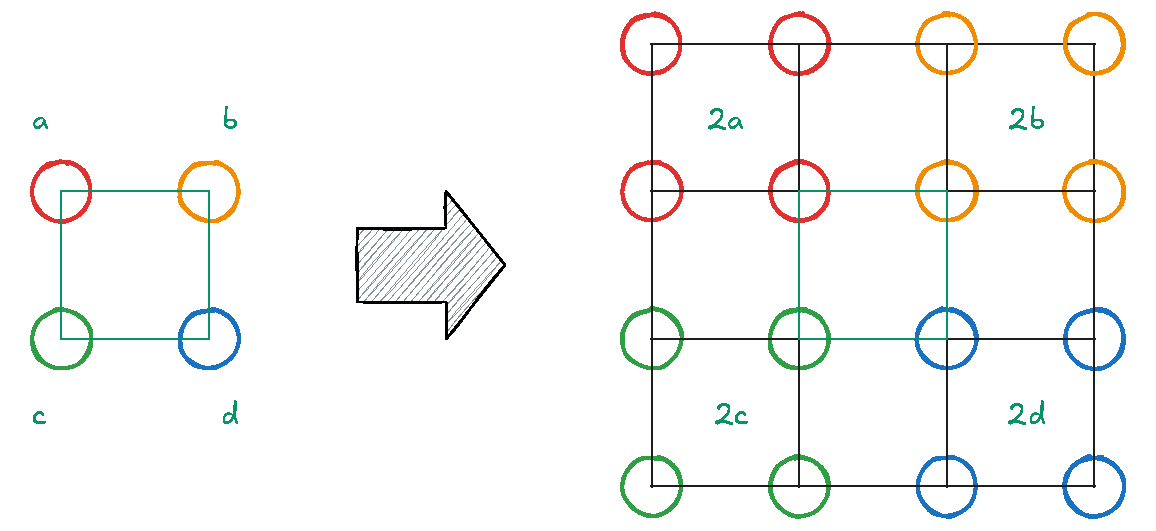
\includegraphics[width=0.7\textwidth]{Chapter3/dim-doubling.pdf}
            \caption{Dimension doubling. We demonstrate the example in two dimensions.}
            \label{fig:chap-3:dim-double}
        \end{figure}
        Moreover, we can make the following observation:
        \begin{align*}
            \forall (2p_i)_{i \in [n]} \in (\{0,1\}^{k+1})^n, b \in \{0,1\}^n & :\Lambda((2p_i + b)_{i \in [n]})\,                                                              \\
                                                                              & = \lambda\left(\left(\left\lfloor\frac{2p_i + b + 1}{2} \right\rfloor\right)_{i \in [n]}\right) \\
                                                                              & = \lambda\left(\left(\left\lfloor p_i + \frac{b + 1}{2} \right\rfloor\right)_{i \in [n]}\right) \\
                                                                              & = \lambda\left((p_i + b)_{i \in [n]}\right)                                                     \\
        \end{align*}
        Which implies that the cube anchored at $p$ must also be panchromatic.
    \end{proof}
    To ensure that $\Lambda$ is hazard free we can use the corollary \ref{col:k-bit-haz}, where we can create an
    $n$-bit hazard-free circuit. One must observe that even though, the size of the circuit increases exponentially
    with respect to the dimensions, but since all the input instances scale with respect to the width of the hypercube space,
    that would imply that we are able to keep the size of the circuit polynomial.
    We therefore claim that this reduction is polynomial and can parsimoniously find all panchromatic cubes.
\end{proof}



\begin{definitionbox}{Kleene Unary Numbers}{kleene-unary}
    \label{def:kleene-unary}
    Given a number $p \in M$, its unary representation can be depicted as a binary number $\{0,1\}^M$ such that: $k \in M \to 1^k \in \bar{M}$.
    Under Kleene algebra, we mainly refer to notations $M_k^n$ where $k,n,M \in \mathbb{N}_0$  such that:
    $$
        M^n_k \triangleq \bigtimes_{i \in [n]} \{1^j\bot^k \mid \forall j \in \mathbb{N}_0 : j + k \leq M\}
    $$
    For a cleaner notation, given $1^j\bot^k \in M_k$ we denote  it as $j\bot^k$.
\end{definitionbox}

For examples of the above notation we refer to the following table:
\begin{table}[h!]
    \centering
    \begin{tabular}{|c|c|}
        \hline
        \rowcolor[HTML]{EAE1E1}
        {\color[HTML]{333333} \textbf{Kleene Unary Sets}} & {\color[HTML]{333333} \textbf{Member examples}} \\ \hline
        $3_1^2$                                           & $(11\bot, 1\bot0) = (2\bot, 1\bot)$             \\ \hline
        $5_0^3$                                           & $(11000, 11110, 11111) = (2, 4, 5)$             \\ \hline
        $7_2^1$                                           & $11\bot\bot000 = 2\bot^2$                       \\ \hline
    \end{tabular}
    \caption{Kleene Unary Examples}
    \label{tab:chap-3:kleene-unary}
\end{table}


\begin{definitionbox}{\scn{HF-StrongSperner} problem}{hf-strong-sperner}
    \textbf{Input}: A hazard-free circuit $\lambda: [M]^n \to \{-1, +1\}^n$, where $M \in n^{O(1)}$ that describes a \textit{StrongSperner} labelling,
    as explained in \ref{def:strong-sperner}, where the inputs are represented using Kleene Unary numbers \ref{def:kleene-unary}.\\
    \textbf{Output}: A point $p \in M_{\leq 1}^n$ if and only if: $\lambda(p) =  \bot^n$.
\end{definitionbox}

We will mainly focus on subproblems of the \textit{HF-StrongSperner} where two cubes do not overlap with each other.
We will use figure \ref{fig:chap-3:overlapping-sperner-solutions} for reference.
Essentially if an edge or a face of a cube result in a solution then, it may cause two issues.
One is that the
More formally we define


\begin{figure}[h!]
    \centering
    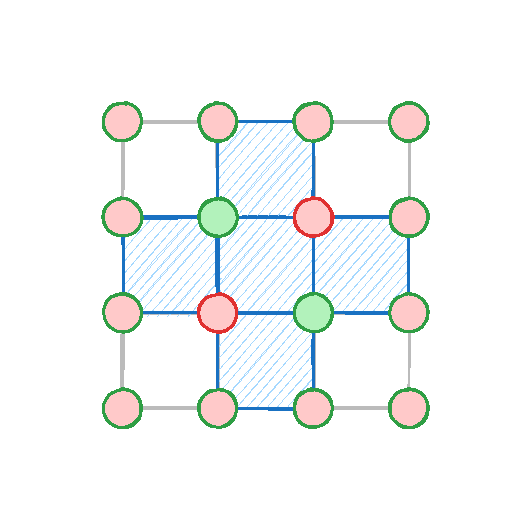
\includegraphics[width=0.7\textwidth]{Chapter3/non-discrete-sperner-colouring-example.pdf}
    \caption{Overlapping Sperner Solutions}
    \label{fig:chap-3:overlapping-sperner-solutions}
\end{figure}


\begin{definitionbox}{\scn{HF-DiscreteStrongSperner} problem}{hf-strong-sperner}
    An \textit{HF-StrongSperner} instance $\lambda$ such that $\forall p \in [M_1]^n$, if $\lambda(p)= \bot^n$, then
    $$
        \forall y \in (\{0,1\}^M)^n: x \preceq y \implies y \text{ does satisfy the labelling condition \ref{def:bipolar-colouring}}
    $$
    Essentially, any subspace of the cube should not yield a panchromatic solution.
\end{definitionbox}

Lastly we introduce a specific subset of the above solutions where introduce antipodal panchromatic cubes.
In the specific type of solution said we argue that two opposite corners of a cube contain opposite colourings.
This notion of antipodal cubes is used in the majority of reductions across literature. More formally we say


\begin{definitionbox}{\textbf{MinRes} min and max resolution functions}{min-res-func}
    We use the \textbf{MinRes}, to denote the smallest resolution of a kleene string. More formally we can use the following equivalent definitions:
    \begin{align*}
        \forall x \in \{0,1,\bot\}^*, j \in [|x|]:  [\textbf{MinRes}(x)]_j
         & \triangleq \begin{cases}
                          x_i & \text{if } x_i \in \{0,1\} \\
                          0   & \text{otherwise}
                      \end{cases}
    \end{align*}
    For the maximum resolution we will use the $\textbf{MaxRes}$ function where we instead replace all $\bot$ with $1$ instead.
\end{definitionbox}

\begin{definitionbox}{\scn{HF-AntipodalStrongSperner} problem}{hf-strong-sperner}
    An \scn{HF-DiscreteStrongSperner} instance $\lambda$ such that $\forall p \in [M^1]^n$, if $\lambda(p)= \bot^n$,
    and denote $\textbf{MinRes}(x) = \hat{x}$ as the \textit{anchor} of the cube, then:
    $$
        \forall b \in \{0,1\}^n, j \in [n]: [\lambda(\hat{x} + b)]_j = -[\lambda(\hat{x} +  1^n \oplus b)]_j
    $$
\end{definitionbox}

We emphasize that the above class considers the subset of the \textit{Hf-DiscreteStrongSperner}
as the antipodality condition cannot ensure discreteness.

\begin{claimbox}{Antipodal discrete squares}{antipodal-discrete-square}
    Given a panchromatic solution of a \scn{HF-AntipodalStrongSperner} $p$, it must be the case then that:
    $$
        \forall j \in \{-1, 1\}^n, \exists! x \in \textbf{Res}(p): \lambda(x) =  j
    $$
\end{claimbox}

\begin{proof}
    We proof by induction on $n$. Lets assume base case $n = 2$. We can observe that the only satisfying
    cube that is both antipodal and discrete, is some rotation of the following matrix
    $$
        \begin{pmatrix}
            \mp & +   \\
            -   & \pm \\
        \end{pmatrix}
    $$
    Where we denote $+ = (+, +), -=(-,-), \pm = (+,-)$ and $\mp = (-,+)$, we can observe indeed that the panchromatic square contains all the colourings.
    For the induction step, we can observe that if we want our colouring function to be both discrete and antipodal, then the following must suffice:
    given $k, k'$ the two resolutions of dimension $k+1$, we know that $[\lambda(p_{-(n+1)}(k))] = (b, \bot^n)$ for some $b \in \{0,1\}^n$. But that implies
    $[\lambda(p_{-(n+1)}(k'))] = (\bar{b}, \bot^n)$, which indicates a discrete antipodal panchromatic solution. Moreover if $p_{-(n+1)}$ cover $2^n$ labels,
    then the whole cube covers all $2^{n+1}$ labels, which by pigeonhole principle means that we must cover all possible combinations of colourings.
\end{proof}



All the problems above are clearly in \textbf{PPAD} as all of them reduce to the \textit{StrongSperner} problem,
since we assume by construction that they \textit{natural} and therefore behave as normal binary circuits. For the purposes of our current
research, we demonstrate a parsimonious reduction from \scn{HF-DiscreteStrongSperner} to \scn{PureCircuit}.


\begin{theorembox}{}{hf-discrete-to-pure}
    $$
        \textbf{\#PPAD}(\scn{HF-DiscreteStrongSperner}) \subseteq \textbf{\#PPAD}(\scn{PureCircuit})
    $$
\end{theorembox}

\begin{proof}
    Given an input instance $\Lambda$ of a \scn{HF-DiscreteStrongSperner}, we create a \scn{PureCircuit}
    \textit{Input nodes}, \textit{Output nodes}, \textit{Bit generator gadget} and \textit{Circuit application gadget}. To visualise our
    construction we will refer to the figure in \ref{fig:chap-3:pure-circuit}. Each of these parts describe the following:
    \begin{enumerate}
        \item  \textbf{Input nodes}: Vector of $n$ value nodes. Will be represented as $(x_i)_{i \in [n]} \in \mathbb{T}^n$.
        \item  \textbf{Bit generator gadget}: Given a value node $x_i$, apply the \textit{Bit generator} gadget such that we
              create Kleene unary number as defined in \ref{def:kleene-unary}, where $x^i \in M^{\leq 1}_n$. We will refer
              to the bit generator circuit as $C_i$.
        \item  \textbf{Circuit application gadget}: Since the above numbers form coordinates in a
              $[M]_0^n$ space, we apply the $\Lambda$ function to extract a set of output nodes $(u^i)_{i \in [n]} \in \gls{kleene-set}^n$.
        \item  \textbf{Output nodes}: We use the \texttt{Copy} gate to copy $u^i \to x_i$, for all $i \in [n]$.
    \end{enumerate}
    The 1st and last part of our construction is self-explanatory, we will analyse the other two sections in greater depth
    and prove some claims.

    \begin{figure}[h!]
        \centering
        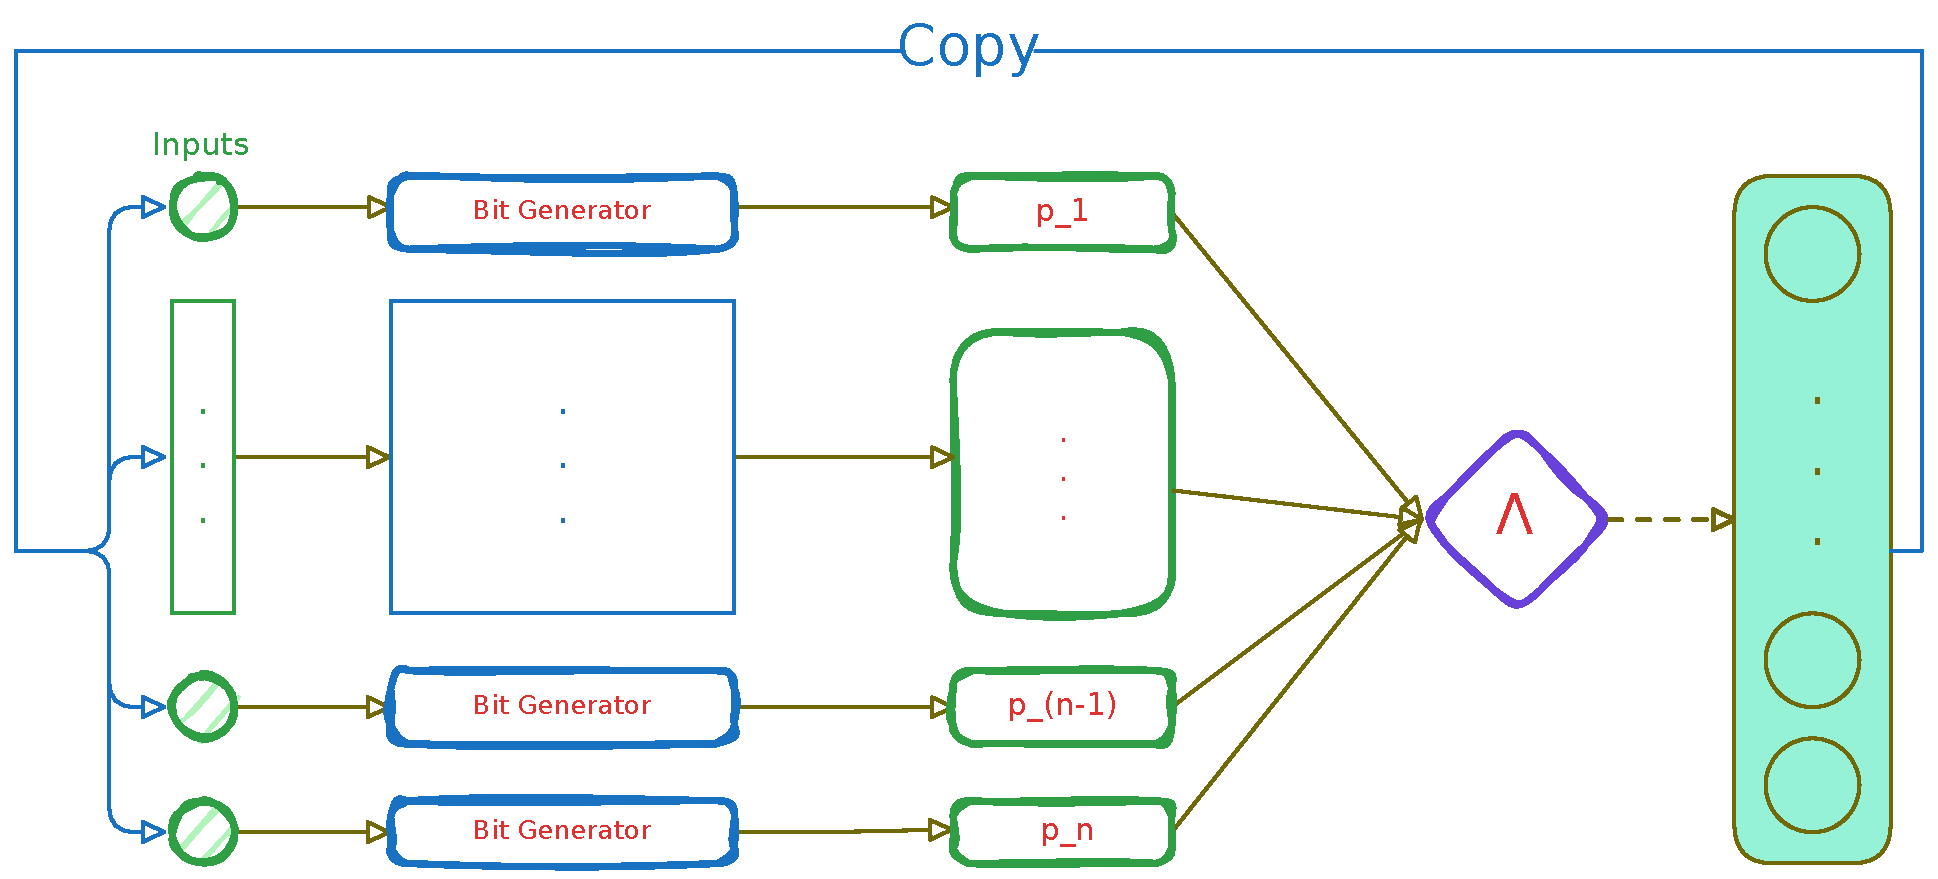
\includegraphics[width=0.5\textwidth]{Chapter3/pure-circuit-reduction.pdf}
        \caption{Pure Circuit construction visualisation}
        \label{fig:chap-3:pure-circuit}
    \end{figure}
    %% TODO reword 
    \paragraph*{Bit generator gadget} In order to create Kleene unary numbers we make use of a binary tree of \texttt{Purify} gates
    as seen in the figure \ref{fig:chap-3:purification-gadget}. We now claim that the current construction has certain desirable properties.


    \begin{figure}[h!]
        \centering %% TODO check the ordering of the graph
        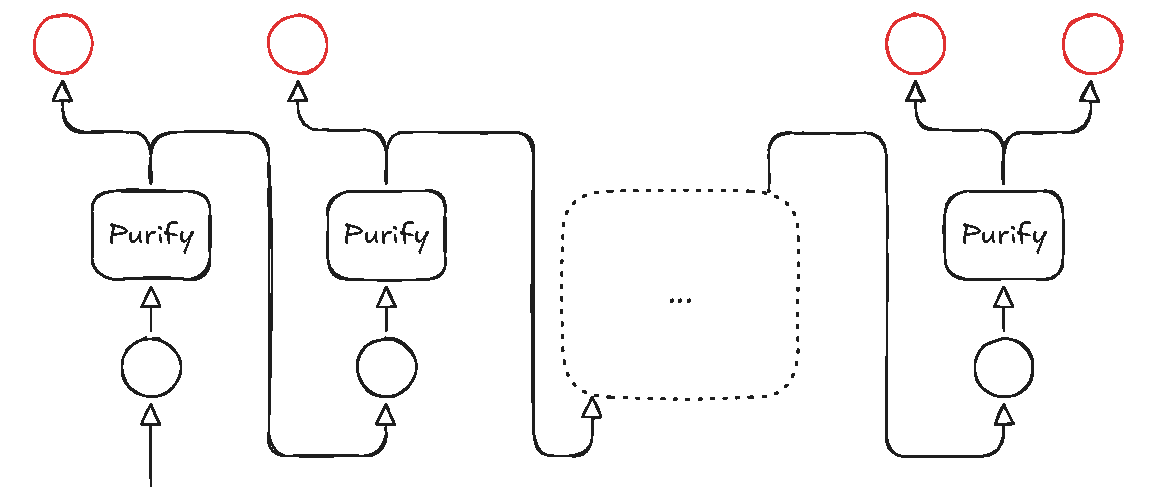
\includegraphics[width=0.5\textwidth]{Chapter3/purification-stage-construction.pdf}
        \caption{Purification gadget. The red nodes denote the outputs of the purification gadget.}
        \label{fig:chap-3:purification-gadget}
    \end{figure}

    \begin{claimbox}{Purification Claim}{chap-3:pur-claim}
        \label{clm:chap-3:pur-claim}
        Given the description of the bit generator gadget, we make the following two claims:
        \begin{enumerate}
            \item $b \in \{0,1\}^n: C_i(b) = b^n$
            \item $C_i(\bot) \in M^{\leq 1}_n$
        \end{enumerate}
    \end{claimbox}
    \begin{proof}
        From the definition of the \texttt{Purify} gate we know that
        $\forall b \in \{0,1\}: \texttt{Purify}(b) = (b,b)$, and therefore any subtree that takes a pure input, will copy its value
        to all its leafs, which follows our first claim directly. To the second part of our lemma, we can observe that
        the only valid outputs are $(0, \bot), (\bot,1), (0,1)$. Based on our previous observation, if a purify gate outputs
        a $(0, \bot)$ value, it will propagate $\bot$ to the rest of the tree and return $0$ in the current level,
        if the value is $(\bot/0, 1)$, the tree will return $\bot/0$ at the specific level, and then propagate $1$ to the rest of the leaves.
        This shows that all possible strings generated are of the form $1^k\bot^{0 \mid 1}0^{*}$.
    \end{proof}


    \paragraph*{Correctness and parsimonious argument}
    One can observe that the current construction is a valid construction, as we satisfy the arities of all gates and ensured
    that every node has an in-degree of $1$. We now make the following lemma

    \begin{lemmabox}{Correctness Lemma}{pure-correct-lem}
        A correct assignment corresponds to panchromatic cube in the original problem instance.
    \end{lemmabox}

    It suffices to show that every vector $x^i \in M^1_\bot$ and $\forall i \in [n]: \mathbf{x}[u^i] = \bot$.
    Assume that we have a correct assignment, and WLOG $\mathbf{x}[u^i] = 0$  for some $i \in [n]$.
    By our copy that, we know that $\mathbf{x}[u^i]= \mathbf{x}[x_i]$.
    By our  purification lemma {..} we know that $\mathbf{x}[x^i] = 0^i$.
    Since our circuit is hazard-free and applies the boundary conditions of the sperner problem, we know that
    $[\Lambda(x_{-i}(0))]_i = 1\neq \mathbf{x}[u^i]$. We can make a similar argument for $\mathbf{x}[u^i] = 1$.
    Therefore, a satisfying assignment corresponds to some panchromatic solution. Given that
    our instance is in \scn{HF-DiscreteStrongSperner}, it has to be the case that
    all $x_i \in M^1_n$, otherwise that would imply that there exists a $(n-1)$-subspace that also covers all the labels.
    This also shows that there exists a 1-to-1 mapping between a panchromatic cube and a satisfying assignment.
\end{proof}

Although the above reduction also works for the general $\textbf{HF-StrongSperner}$, the reduction is not parsimonious since
the \textit{PureCircuit} will accept solutions for all $(n-1)$ subspaces that contain a covering set. %% TODO


Unfortunately, showing hardness is a much harder task.
In the paper
\cite{chen_SettlingComplexityComputing_2009} they showed that given $f(n) \in O(n)$,
they demonstrated how one can apply the \textit{Snake Embedding} technique
where one can fold the space in higher and higher dimensions
with the goal of going from a $2^n \times 2^n$ space to  $f(n)^m$  where $m, f(n) \in O(n)$. The original reduction,
expresses the ability to go from a $2^n \times 2^n$ space, to a $[2^f(n)]^d$ where $d = \lceil \frac{n}{f(n)} \rceil$ space,
where $f(n)$ is some well-defined polynomial function that grows linearly or less.
We know that \textit{EndOfLine} can parsimoniously reduce to the \textit{2D-StrongSperner} problem,
and as we will demonstrate in the later sections, using their snake embedding technique, the
number of solutions will be preserved per folding. The problem is that we cannot guarantee,
the hazard-freeness property of every fold.
If we try to use the  corollary 10 by \cite{ikenmeyer_ComplexityHazardfreeCircuits_2019},
we observe that the circuit size will increase exponentially. This implies the best we can hope for
when using their method is:
$$
    M = n^k, f(n) = \log_2(n)^k \implies d = \frac{n}{log(n)^k}
$$
In the upcoming sections, we propose a chain of parsimonious reductions from the \textit{EndOfLine}
to \textit{AntipodalStrongSperner}. We emphasize that this method will still not be hazard-free,
but we hope that the antipodal properties of resulting problem may enable for a full reduction in the future.
We will start with the \textit{Bipolar colouring} of \textit{RLeafD}, where we extend
the colouring of Chen et al. \cite{chen_Complexity2DDiscrete_2009}.

\paragraph*{Bipolar colouring of \textit{RLeafD}}

We construct the same reduction as in the \textit{RLeafD} but with slight differences:
We will use points $\mathbf{u}, \mathbf{v}, \mathbf{w} \in V_{2^k}$ and $\mathbf{p},\mathbf{q}, \mathbf{r} \in B_{2^{4k+10}}$ where
$$
    B_n \triangleq [n]_0 \times [n]_0
$$
Moreover a polychromatic square will be denoted if all the points in the neighbouring squares satisfy the bipolar colouring.
Morevoer below we will denote our colouring scheme for clarity:
\begin{align*}
    +   & = (+1, +1) \\
    \pm & = (+1, -1) \\
    \mp & = (-1, +1) \\
    -   & = (-1, -1) \\
\end{align*}


First, we define mapping $\mathcal{F}: V_{2^k} \to B_{2^{4k+10}}$ such that %TODO: Careful about edges
$$
    \mathcal{F}(\mathbf{u}) = \begin{pmatrix}
        6 \mathbf{u}_{1} + 6 \\
        6 \mathbf{u}_{2} + 6 \\
    \end{pmatrix} \in B_{2^{4k+10}}
$$
Since $G \in C_{2^k}$, its edge-set can be decomposed into a collection of paths and cycles $(P_{i})_{i \in [m]}$.
By using $\mathcal{F}$, every $P_{i}$ is mapped to a set $I(P_{i}) \subset B_{2^{4k+10}}$
We will colour every point  on $I(P_{i})$ with $+$
\begin{gather}
    P = \mathbf{u}^1,\dots,\mathbf{u}^t \text{, if P is a cycle } \mathbf{u}^1 = \mathbf{u}^t \\
    I(P) \triangleq \bigcup_{i \in [t-1]} I(u^tu^{t-1})
\end{gather}
A lot of \textit{Line reductions} under colouring use the notion of shielding. %% TODO add references to all problems
Essentially we embed our lines and cycles in a grid, everything not a line is denoted as a negative charge $-$.
All lines are denoted as positive charge $+$. To protect our lines from creating solutions, we cover them
with $\pm, \mp$ lines. A visualisation can be seen in figure \ref{fig:chap-3:eol-shielding}.
We define the following set to denote the set of shielding points around our paths.

$$
    O(P) = \{  \mathbf{p} \in B_{2^{4k+10}} \setminus I(P) :\mid: \exists \mathbf{p}' \in I(P), \|p- p'\|_{\infty} = 1 \}
$$

\begin{figure*}
    \centering
    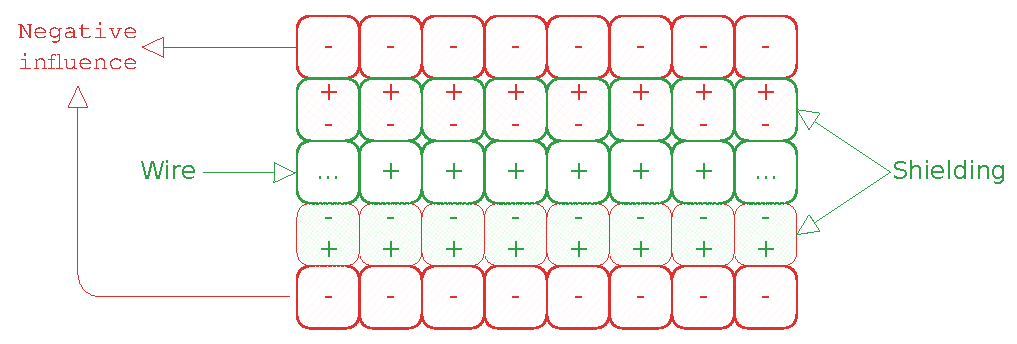
\includegraphics[width=0.5\textwidth]{Chapter3/coiling-eol.pdf}
    \caption{Shielding method on 2D-EoL embeddings.}
    \label{fig:chap-3:eol-shielding}
\end{figure*}
If $P$ is a simple path we can decompose $\{ \mathbf{s}_{p}, \mathbf{e}_{p} \} \cup L(P) \cup R(P)$ such that:
$\mathbf{s}_{p} = \mathcal{F}(\mathbf{u}^1) + \Delta + \Delta^\perp$, where $\Delta = (\mathbf{u^1}- \mathbf{u}^2)$,
$\mathbf{e}_{p} = \mathcal{F}(\mathbf{u}^1) + \bar{\Delta} + \bar{{\Delta}}^\perp$, where $\bar{\Delta}= (\mathbf{u}^t - \mathbf{u}^{t-1})$
and $x^\perp$, denotes the vector perpendicular to $x$. Choice of which perpendicular vector we consider is arbitrary.
Starting from $\mathbf{s}_{p}$,
enumerate vertices in $O(P)$ clockwise as $\mathbf{s}_{p},\mathbf{q}^1,\dots,\mathbf{q}^{n_{1}}, \mathbf{e}_{p}, \mathbf{r}^1,\dots,\mathbf{r}^{n_{2}}$ such that
\begin{align*}
    L(P) & = \{ \mathbf{q}^i \}_{i \in [n_{1}]}\ , \\
    R(P) & = \{ \mathbf{r}^i \}_{i \in [n_{2}]}\,  \\
\end{align*}
If $P$ is a simple cycle, then can can decompose $L(P) \cup R(P)$, where $L(P)$ contains all the vertices on the left side of the cycle and $R(P)$ all the vertices on the right side
If $G$ is specified by $(K, 0^k) \subset C_{2^k}$, we can uniquely decompose the edge set into $P_{1}, \dots P_{m}$
Every path is either a maximal path, or a cycle in $G$.
We can use the following to describe our colouring algorithm:

\begin{algorithm}
    \caption{Turing machine $F$ with input $(p_1, p_2) \in B_{2^{4k+10}}$}
    \begin{algorithmic}
        % \If{$p_1 = 0$}
        %     \If{$p_2 \leq 6$}
        %         \Return $+$
        %     \Else
        %         \Return $\pm$
        %     \EndIf
        % \Elsif{$p_1 < 6$}
        %     \If{$p_2 = 6$}
        %         \Return $+$
        %     \Elsif{$p_2 < 6$}
        %         \Return $\mp$
        %     \Elsif{$p_2 = 7$}
        %         \Return $\pm$
        %     \Else
        %         \Return $-$
        %     \EndIf
        % \EndIf
        % \Return $M_K(\mathbf{p})$
        \If{$p_1 = 0$}
        \If{$p_2 \leq 6$}
        \State \Return $+$
        \Else
        \State \Return $\pm$
        \EndIf
        \ElsIf{$p_1 < 6$}k
        \If{$p_2 = 6$}
        \State \Return $+$
        \ElsIf{$p_2 < 6$}
        \State \Return $\mp$
        \ElsIf{$p_2 = 7$}
        \State \Return $\pm$
        \Else
        \State \Return $-$
        \EndIf
        \Else
        \State \Return $M_K(\mathbf{p})$
        \EndIf
    \end{algorithmic}
\end{algorithm}

Where $M_{k}(\mathbf{p})$ is can be described with the following description:
$$
    M_{k}(\mathbf{p})  =\begin{cases}
        +   & \text{ if } \exists i, \mathbf{p} \in I(P_{i})                \\
        \pm & \text{ if }\exists i, \mathbf{p} \in L(P_{i}) \vee p_{1} = 0  \\
        \mp & \text{ if } \exists i, \mathbf{p} \in R(P_{i}) \vee p_{2} = 0 \\
        -   & \text{ otherwise}
    \end{cases}
$$
We will call the path of nodes $(0,0) \to (0,6) \to(6,6)$ as the tail, which
ensures that the $0^n$ node of our original graph is not a solution.
An example of how such reduction looks like can be seen in figure \ref{fig:chap-3:eol-sperner-colouring}.
\begin{figure}[h!]
    \centering
    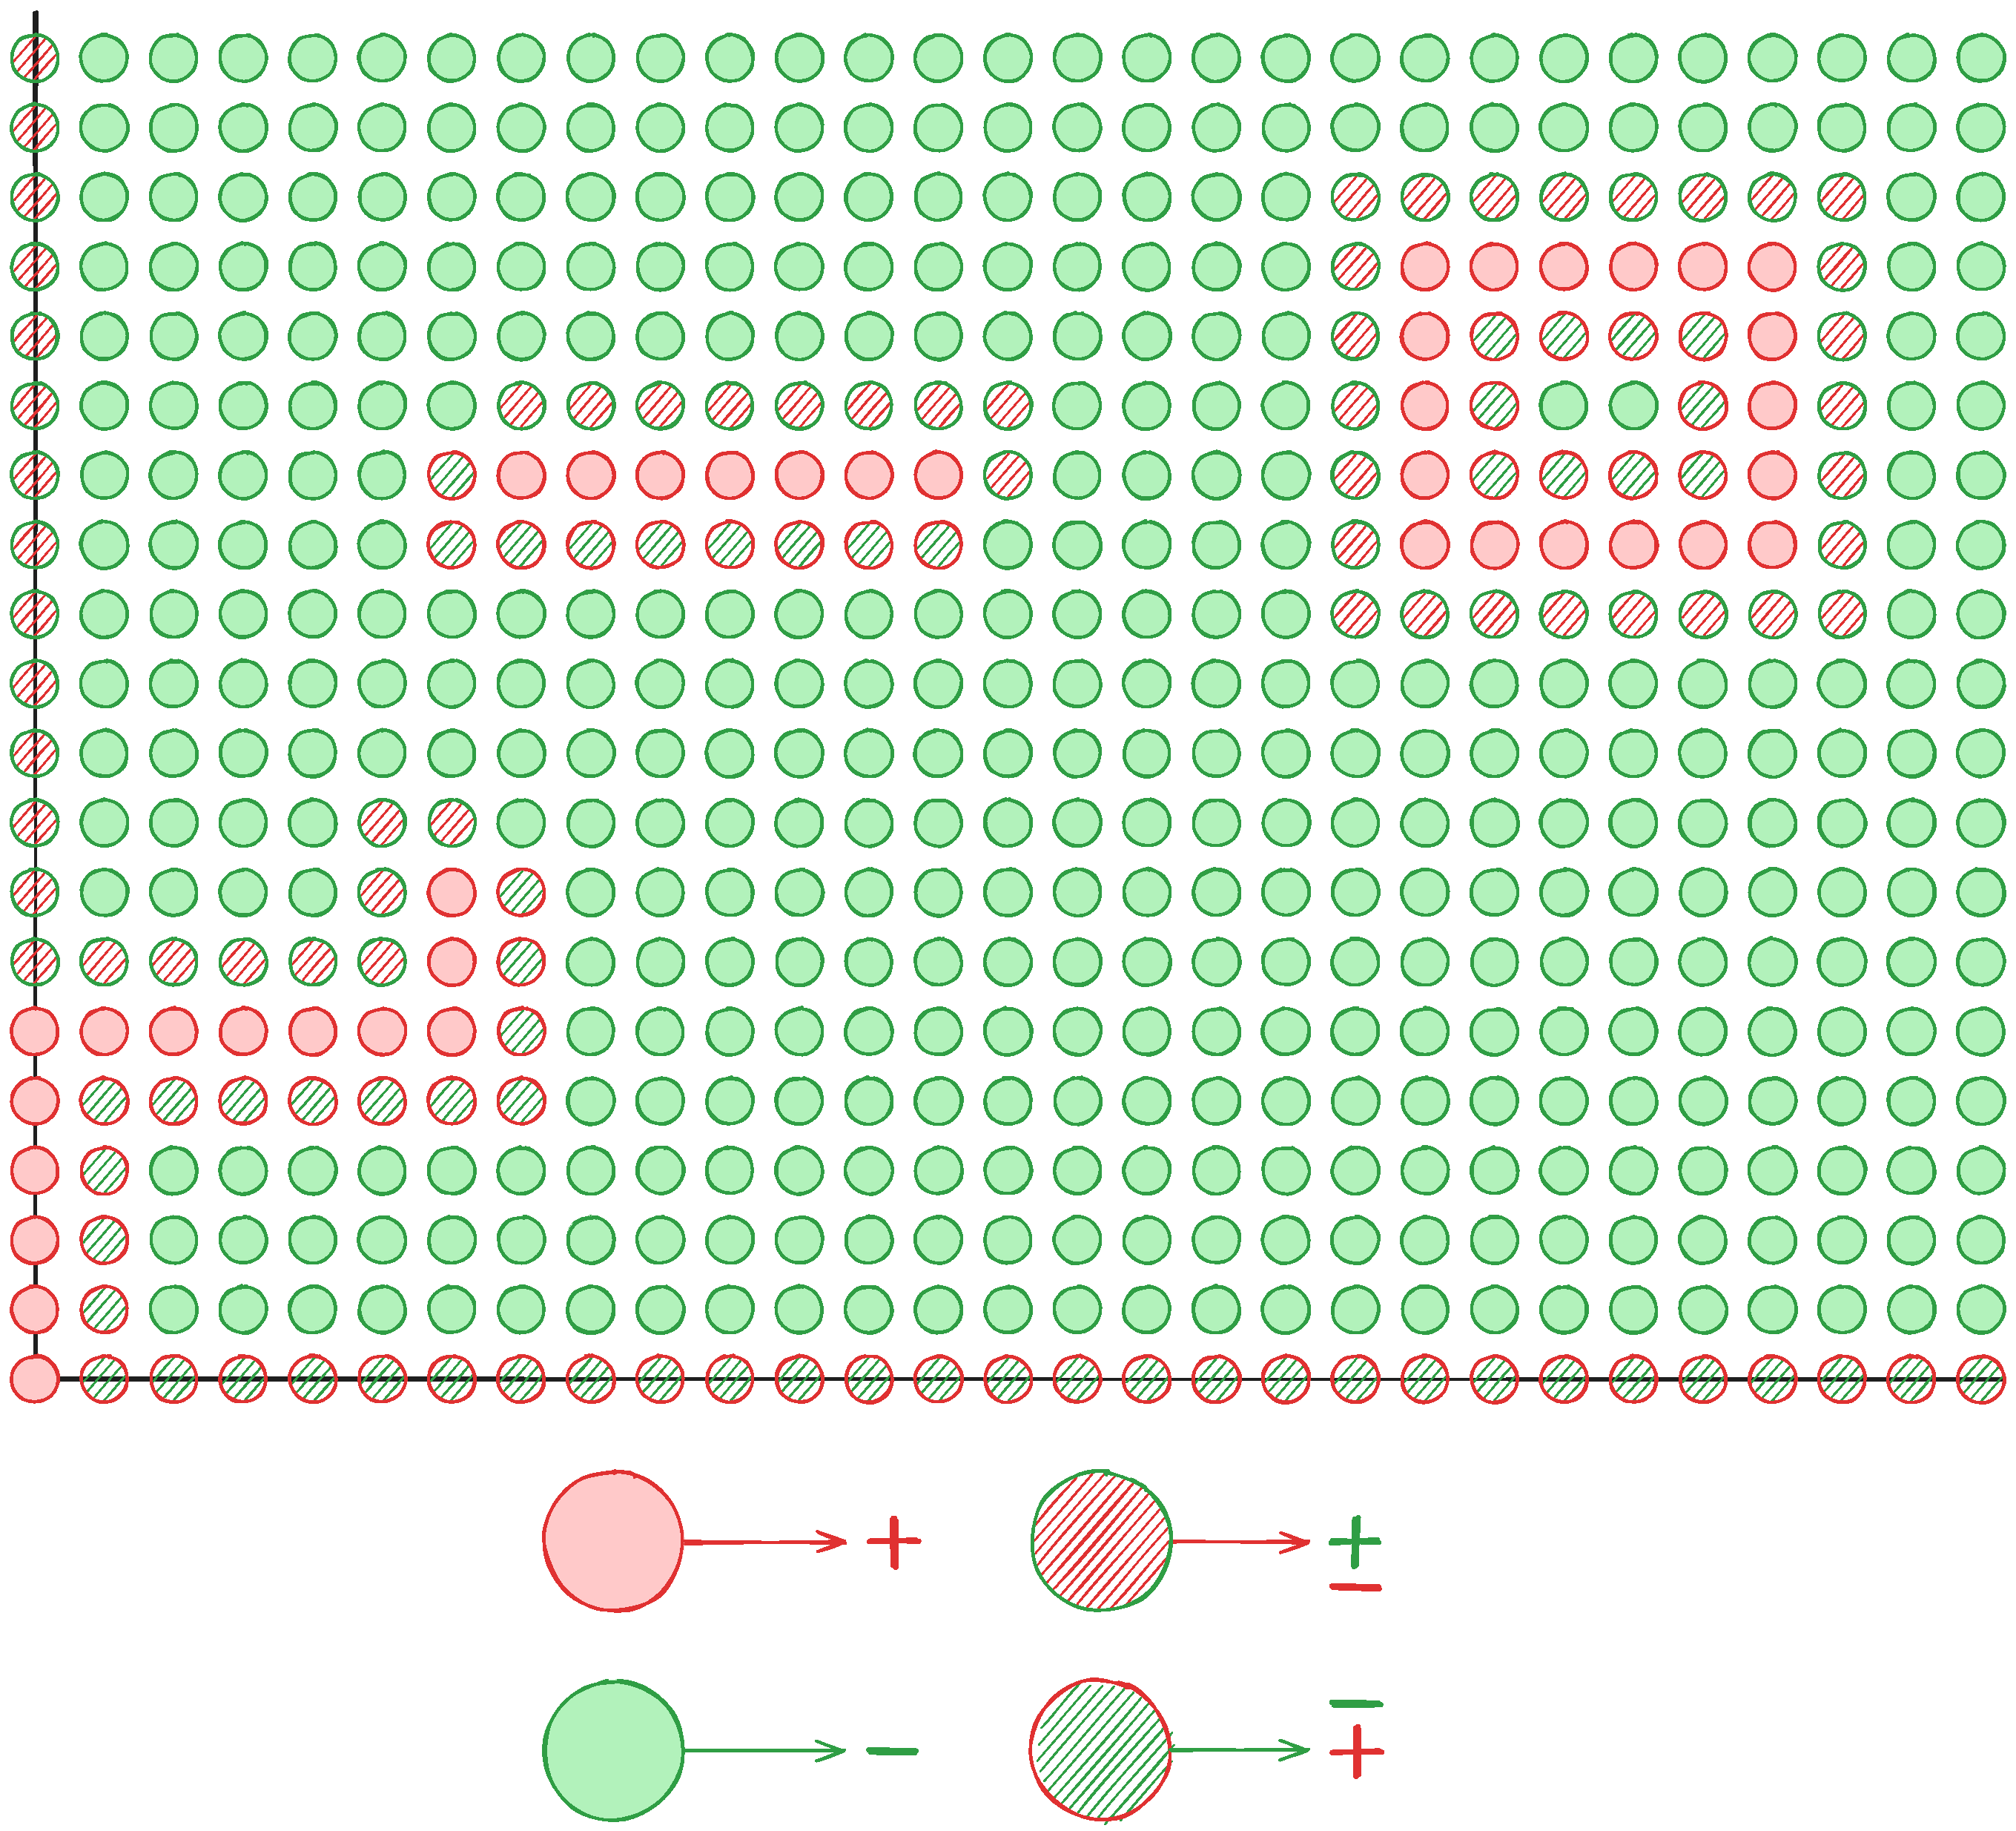
\includegraphics[width=0.5\textwidth]{Chapter3/2d-sperner-eol.pdf}
    \caption{2D EndOfLine Bipolar Colouring}
    \label{fig:chap-3:eol-sperner-colouring}
\end{figure}


\begin{lemmabox}{Correctness Lemma}{2d-eol-corr-lemma}
    The following statements hold correct:
    \begin{enumerate}
        \item $\forall i,j: \min_{x \in P_{i}, y\in P_{j}} \|\mathcal{F}(x) - \mathcal{F}(y) \|_{\infty} > 4$
        \item All polychromatic squares represent solutions
    \end{enumerate}
\end{lemmabox}

To prove the first statement, assume we have  $a,b \in V_{2^k}: \|a - b\|_{\infty} \geq 1$. WLOG assume
$a -b = (x,y)$ for some $x,y \in \mathbb{N}$ which implies the following:
\begin{gather*}
    \mathcal{F}(a) = \mathcal{F}\begin{pmatrix}
        b_{x} + x \\
        b_{y} + y \\
    \end{pmatrix} = \begin{pmatrix}
        6b_{x}+6x + 6 \\
        6b_{x}+6y + 6 \\
    \end{pmatrix} \\ \\
    \mathcal{F}(a) - \mathcal{F}(b) =  \begin{pmatrix}
        6x \\
        6y \\
    \end{pmatrix}
\end{gather*}
Since $x + y > 0 \implies \|\mathcal{F}(a) - \mathcal{F}(b)\|_{\infty} \geq 6 > 4$.  This statement is meant space all lines and their shieldings
are far enough from each other such that the colourings will not create additional solutions.
Visually what this looks like is, if we had to parallel lines in $V_{2^k}$, then
the mappings with the colourings, will look like the figure in \ref{fig:chap-3:trans-domain-rleaf}.

\begin{figure}[h!]
    \centering
    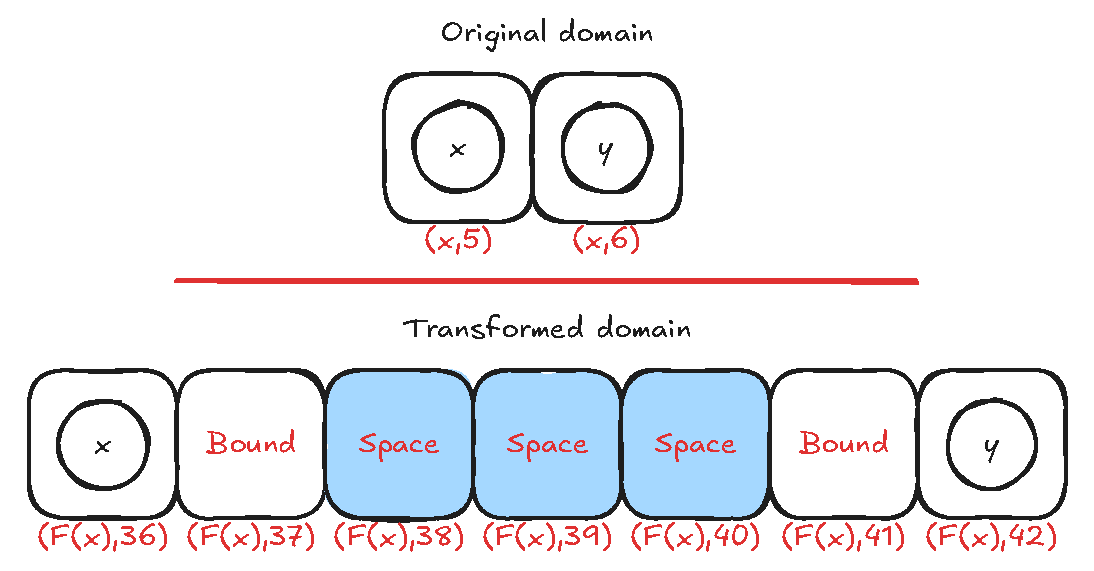
\includegraphics[width=0.7\textwidth]{Chapter3/trans-dom-relfad.pdf}
    \caption{Transformed domain mapping example.}
    \label{fig:chap-3:trans-domain-rleaf}
\end{figure}

% $$
%     \forall i ,j : 1\leq i\neq j \leq m : \Big(I(P_{i}) \cup O(P_{i})\Big) \cap \Big( I(P_{j}) \cap O(P_{j}) \Big) = \emptyset
% $$


To show our second part of our solution, we can observe that:
All nodes that are not boundary not in $\bigcup_{i }I(P_{i}) \cup L(P_{i}) \cup S(P_{i})$ are coloured $-$.
All $+$ coloured nodes are on the tail and in all lines, all non-tail nodes are cushioned by $\pm, \mp$ and every non-tail node is not poly chromatic.
All $-$ elements do not affect $\pm,\mp$  coloured nodes.
Since all lines are sufficiently apart from each other, it suffices to check only the ends of paths, as
for squares in the lines we can observe that we only have labels $\{\pm, +\}$ or $\{\mp, +\}$.
One can observe that the square that contains $s_{P_{i}}$ and the start of a line,
or the square that contains $e_{P_{i}}$ and the end of a line will be polychromatic.
Therefore, we have a valid and parsimonious reduction since we only cubes and the beginnings or ends of lines can be solutions.
We call this coloured instances as \textit{2D-StrongRLeafD}

\paragraph{Going from \textit{2D} to higher dimensions}

We now demonstrate how to go from \textit{2D-StrongRLeafD} to
\textit{AntipodalStrongSperner}. We employ
a slightly adjusted method than one proposed by Chen et al. \cite{chen_SettlingComplexityComputing_2009},
which closely resembles the \textit{Snake Embedding} technique used
by Deligkas et al. \cite{deligkas_ConstantInapproximabilityPPA_2022}
on the \textit{StrongTucker} version of the problem, which reduced the space
from $2^n \times 2^n \to 7^m$, where $m = O(n)$. We will show how to expand their method
for the \textit{StrongSperner} problems as well as demonstrate that
such reduction will resolve in an \textit{AntipodalStrongSperner} instance.


\begin{theorembox}{}{parsimonious-2d-strong-eol-to-antipodalss}
    $$
        \textbf{\#PPAD}(\scn{2D-StrongEoL}) \subseteq \textbf{\#PPAD}(\scn{AntipodalStrongSperner})
    $$
\end{theorembox}

\begin{proof}

    General idea is that we have these twisted sheets that capture the $n-1$ embedding onto the higher on
    We are given as an input a $2^n \times 2^n$ grid representing any \textit{2D-StrongEoL} problem.
    The procedure is summarised as follows:
    Given dimension $n$, apply the \textbf{padding operation} such that $n' = 3 \cdot s + 1$ for some $s \in \mathbb{N}$.
    Then apply the \textit{folding} operation, which reduces ``width'' of the space to
    $s + 3$ and compresses the space into a higher dimension. This resembles
    how we can take a sheet of paper and fold it half way such that it now has a third dimension,
    but a smaller width on the folded one. We will now go into a greater detail as to how each operation works.
    To make notation simple and consistent, we define $M^t$ as
    $$
        M^t \triangleq  \bigtimes_{i \in [n_t]} m_i^t
    $$
    Where $m_i^t$ denotes the width of dimension $i$ at iteration $t$, and $n_t$ as the number of dimensions.

    \paragraph*{Padding Dimensions} We will use the definition \ref{def:pad-dim-op} to define our operation.

    \begin{definitionbox}{Padding dimension $P(T,i,u)$}{pad-dim-op}
        \label{def:pad-dim-op}
        Given labelling function $\Lambda^t: M^t \to \{-1,+1\}^{n_t}$, we define
        the padding operation $P(\Lambda^t, i, u)$ for $i \in [n_t]$ and $u \in \mathbb{N}$ where
        $n_{t+1} = n_t$ and
        $$
            \forall j \in [n_{t+1}]: m_j = \begin{cases}
                m_i     & \text{if }  i \neq j \\
                m_i + u & \text{otherwise}
            \end{cases}
        $$
    \end{definitionbox}

    The above operation extends dimension $i$ with $u$ additional layers.
    How the operation work is that we append a \textit{null} dimension such that,
    given $\bar{x} = x_{-i}(m_i^t + 1)$:
    $$
        \forall x \in M^t, j \in [n] : [\Lambda^{t+1}(\bar{x})]_j  = \begin{cases}
            -1 & \text{if } \bar{x}_i > 0 \\
            +1 & \text{otherwise}
        \end{cases}
    $$
    We can be sure that the above will not result in any new solutions since
    in $[\Lambda^t(\cdot, m^t_i, \cdot)]_i = -1$, and therefore
    any solution between  $(\cdot, m^t_i, \cdot), (\cdot, m^t_i+ 1, \cdot)$  will not yield in a solution.

    \paragraph{Snake Folding} below we will give a overview of the snake folding operation.
    Before giving a formal definition, we will first give an informal overview of what
    the technique actually does based on the figure \ref{fig:chap-3:snake-embedding-visualisation-basic}.
    The $y$-axis denotes the new dimension, denoted as $d'$ and the $x$ axis denotes the folded dimension
    referred as $\bar{i}$ with width $m_{\bar{i}}^{t+1} = s + 3 = m_{\bar{i}}^{t'}$,
    given that the original width was $3s+1$ for some $s \in \mathbb{N}$.
    Moreover, we will use notation $(a, b)$ as $a$, the labels in the
    $n_t$ subspace and $b$ as the label of the $n_t+1$ dimension.
    From the figure we observe that we have orange, red, green and blue lines.
    Blue and orange lines denote $(\omega, -)$ and $(\omega, +)$ where $\omega$
    is the $d$-dim null space, where for each point $>0$, we use label $-$ and for $0$
    we use label $+$. For the red and green lines,
    these are denoted as $(\star, -), (\star, +)$ where $\star$ is an $n$-dim copy of the lower
    space with some additional points. The core idea is that all solutions, must belong in between
    the red and green lines, and if we have a solution in the $n_t$-space, we should also have a
    solution in the $n_t+1$ space, as shown in the figure \ref{fig:chap-3:snake-embedding-2d-to-3d-sol}.


    \begin{figure}[h!]
        \centering
        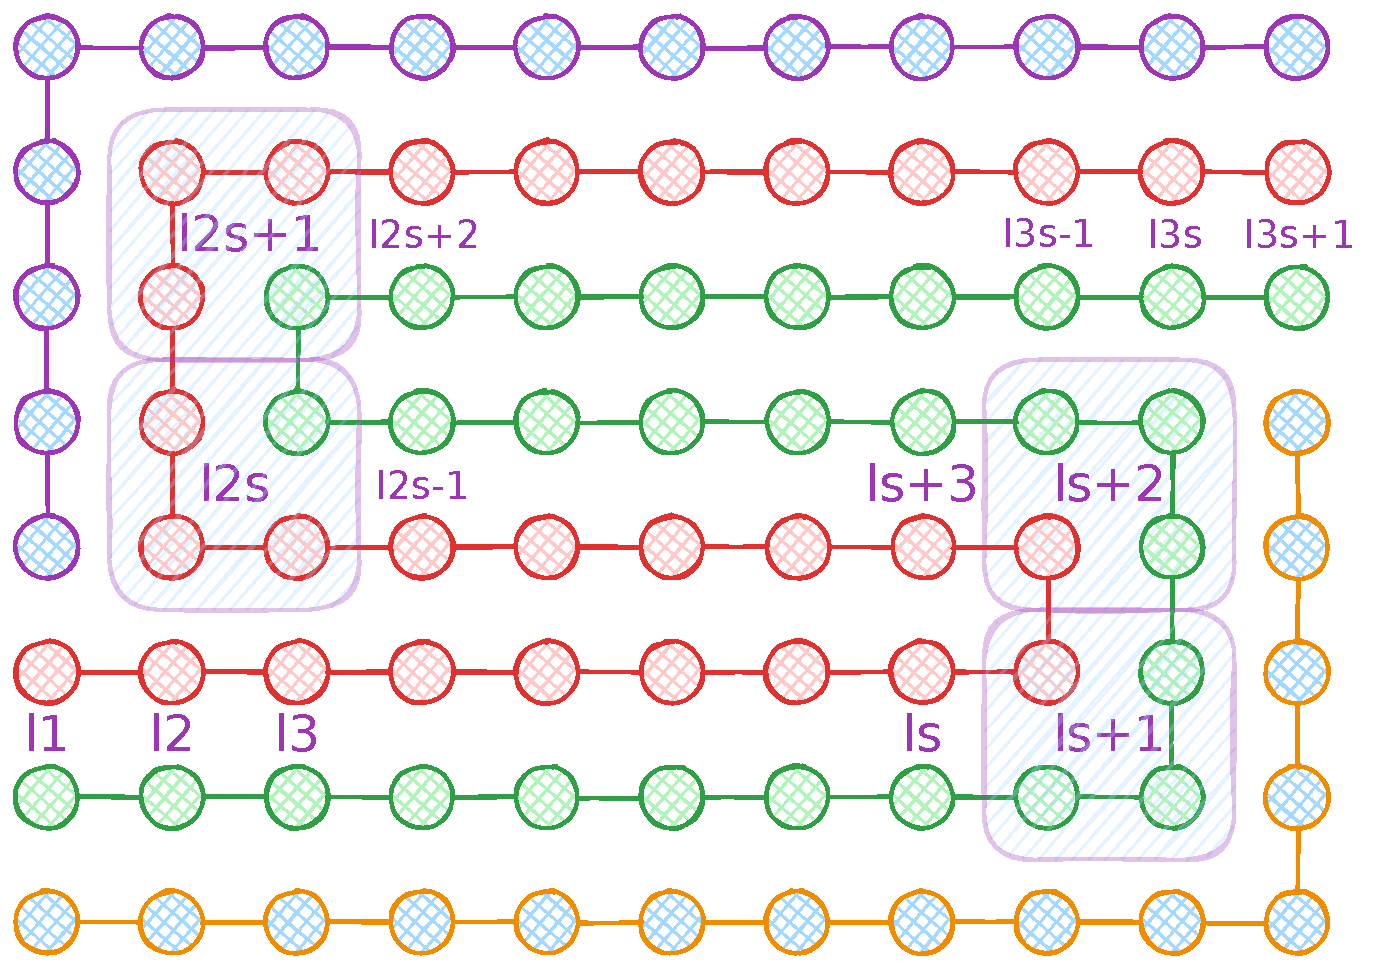
\includegraphics[width=0.7\textwidth]{Chapter3/snake-embedding-simplified.pdf}
        \caption{Snake Embedding technique between the folding dimension and the new dimension}
        \label{fig:chap-3:snake-embedding-visualisation-basic}
    \end{figure}

    \begin{figure}[h!]
        \centering
        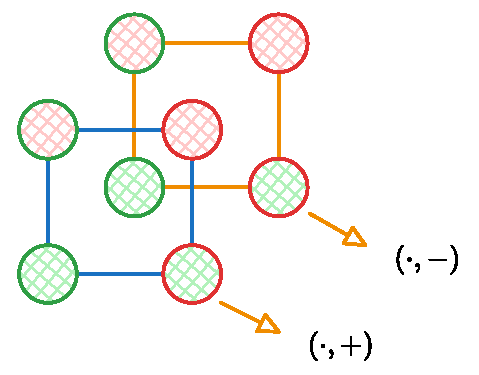
\includegraphics[width=0.5\textwidth]{Chapter3/2d-to-3d-snake-sol.pdf}
        \caption{Snake Embedding technique between the folding dimension and the new dimension}
        \label{fig:chap-3:snake-embedding-2d-to-3d-sol}
    \end{figure}

    To define the above more formally, we define sets $B^U,B^L \subseteq M^{t'}$
    which denote the set of boundary indices of the orange and blue lines.
    In addition, we define functions $\ell^P, \ell^N \subseteq M^{t'}$ to denote the points on the greed and red lines
    with functions $\phi^P, \phi^N$  that are the inverse maps $\phi^i: \ell^i \to M^t$ that indicate the indexes in the original space.
    Given our new circuit $\Lambda^{t+1}$, we define the following:
    $$
        \forall x \in M^{t+1}, j\in [n_t]:  [\Lambda^{t+1}(x)]_j = \begin{cases}
            -1                           & \text{if  }  x \in B^U \cup B^O \wedge x_j > 0 \\
            +1                           & \text{if  }  x \in B^U \cup B^O \wedge x_j = 0 \\
            [\Lambda^{t+1}(\phi^P(x))]_j & \text{if } x \in \ell^P                        \\
            [\Lambda^{t+1}(\phi^N(x))]_j & \text{if } x \in \ell^N                        \\
        \end{cases}
    $$
    For the new dimension, we apply the labelling rules as described previously
    $$
        \forall x \in M^{t+1}:  [\Lambda^{t+1}(x)]_{n_t+1} = \begin{cases}
            -1 & \text{if  }  x \in B^U \cup \ell^N \\
            +1 & \text{if  }  x \in B^L \cup \ell^P \\
        \end{cases}
    $$
    Using the above we formally define the operation the snake embedding operation $S(T, i)$.

    \begin{definitionbox}{Snake Embedding operation $S(\Lambda^t, i)$}{snake-emb-op}
        Given labelling function $\Lambda: M^t \to \{-1, +1\}^n$, apply the snake embedding operation
        on dimension $i \in [n]$, where $m_i \equiv 1 \mod 3$, to a get a new labelling function
        $\Lambda': M^{t+1} \to \{-1, +1\}^{n+1}$ such that $m'_i = s + 3, n_{t+1} = n_t +1, m_{n_{t+1}} = 7$, where $\Lambda^{t+1}$ is defined
        based on the above description.
    \end{definitionbox}

    \begin{claimbox}{Antipodality Solution preservation}{snake-emb-sol-anti}
        Given operation $S(\Lambda^t, i)$, we argue the following hold true:
        \begin{enumerate}
            \item If $\Lambda^t$ which is antipodal, it will be preserved in the operation.
            \item The number of solutions between the two spaces will be preserved
        \end{enumerate}
    \end{claimbox}

    \begin{proof}
        We observe to the labelling conditions by comparing the original with its folded state.
        Assume we apply the snake folding operation on dimension $j$.
        We can observe that all solutions in the embedded space will be anchored between the red or green lines
        (using figure
        \ref{fig:chap-3:snake-embedding-visualisation-basic}), otherwise the new dimension will not be covered.
        Moreover, one can observe that a panchromatic hypercube can never be anchored in any of the turning points since
        our labelling is discrete and we know that
        any $n_t-1$ subspace cannot yield any panchromatic solutions. Assume we have a point
        in $p \in M^{t+1}$, which is an anchor of some panchromatic solution for some $p_j \in [m^{t+1}_j]$ and
        $p_x \in[m^{t+1}_{n_{t+1}}]$. We can observe from the diagram \ref{fig:chap-3:snake-embedding-visualisation-basic}
        that the coordinates $(\cdot, p_j, p_x)$  correspond to some point $(\cdot, j)$ for some point in the pre-folded space.
        WLOG assume that $(\cdot, j+1)$  corresponds to the point $(\cdot, p_j + 1, p_x)$. That would imply that
        points $(\cdot, p_j, p_x), (\cdot, p_j + 1, p_x)$ yield a panchromatic solution for the $n_t$-dimensional subspace
        up to the first $n_t$-dimensions. In order to cover the $n_{t+1}$-th dimension, we can observe that
        the points $(\cdot, p_j, p_x+1), (\cdot, p_j+1, p_x+1)$  with $(\cdot, p_j, p_x), (\cdot, p_j + 1, p_x)$
        are sufficient to cover all labels. But we can observe that those solutions points are part
        of the $n_{t+1}$-dim cube which implies that we have a panchromatic solution.
        This would also imply that if the $n_t$ subspace of the cube does not cover the first $n_t$ labels, then the folded
        dimension will also not yield any labels, which implies that the number of solutions is preserved between foldings.
        Moreover we can observe that given our previous definition,
        $$
            \forall j \in [n], b \in \{0,1\}^n: [\lambda(p + b0)]_j = [\lambda(p + (1^n \oplus b)0)]_j
        $$
        And
        $$
            \forall b \in \{0,1\}^n: [\lambda(p + b1)]_j = -[\lambda(p + (1^n \oplus b)1)]_j
        $$
        Which implies that our cube is also antipodal
    \end{proof}
    We observed that our operations do not affect the cardinality of solutions. We now outline
    our construction of our new circuit
    \begin{enumerate}
        \item Check if there is a dimension with $m_i^t > 8$. If yes, first pad the dimension such that $m_j^t \equiv 1 \mod 3$.
              Afterwards fold the dimension on $j$ to get new folded circuit
        \item If the folding results in a width of $m_i^t <8$, then we can pad the dimension to have a width of $8$
        \item If no operations were done then we can terminate
    \end{enumerate}
    We can observe that in each step of the algorithm we preserve our solution. Moreover, each fold
    divides the dimension by some factor of $3$. We can therefore observe that the runtime for the creation
    of such circuit will take $O(n\log_32)$. This concludes our proof.
\end{proof}

This is the closest that we manage to bring the reduction chain across \textit{EndOfLine} and \textit{PureCircuit}.
We argue the antipodality property might offer useful properties as we can immediately discern solutions
by looking at antipodal pairs as it is much more computationally efficient than trying to find $d+1$ points in some hypercube
and it doesn't scale with the dimensionality of the space. Unfortunately, we haven't figured a way to exploit,
this property with hazard-free logic and we leave it as a future direction.


Lastly, we observe that throughout literature such as \cite{ikenmeyer_ComplexityHazardfreeCircuits_2019}
and \cite{deligkas_PureCircuitTightInapproximability_2024}, both constructions take advantage of speculative
computing, where we calculate the input on multiple copies of the value and use the result of the majority.
Unfortunately, while this can resolve a lot of the reductions, it may lead to 1-to-many mapping
between the solutions of the original problem domain and the \textit{PureCircuit} domain. %% TODO Might need more look at later
 